\section{Locomotion}
\label{sec:Locomotion}
Soft and continuously deformable locomotion systems can be made from fluidic elastomer body segments.
Specifically, in this section we detail how soft robotic fish can be composed by combining the actuated segments that were presented in Section~\ref{subsec:Actuators, Actuator Morphologies} with a portable power system.

\subsection{Pneumatic Fish}
\label{subsec:Locomotion, Pneumatic Fish}
The soft pneumatic fish developed in \cite{marchese2014autonomous} with a ribbed actuator is shown as a complete system in Figure~\ref{fig:pneumaticfish_system} and performing an escape response in Figure~\ref{fig:pneumaticfish_escape}.

\begin{figure}[htb]
        \centering
        \begin{subfigure}[b]{\columnwidth}
            \centering
            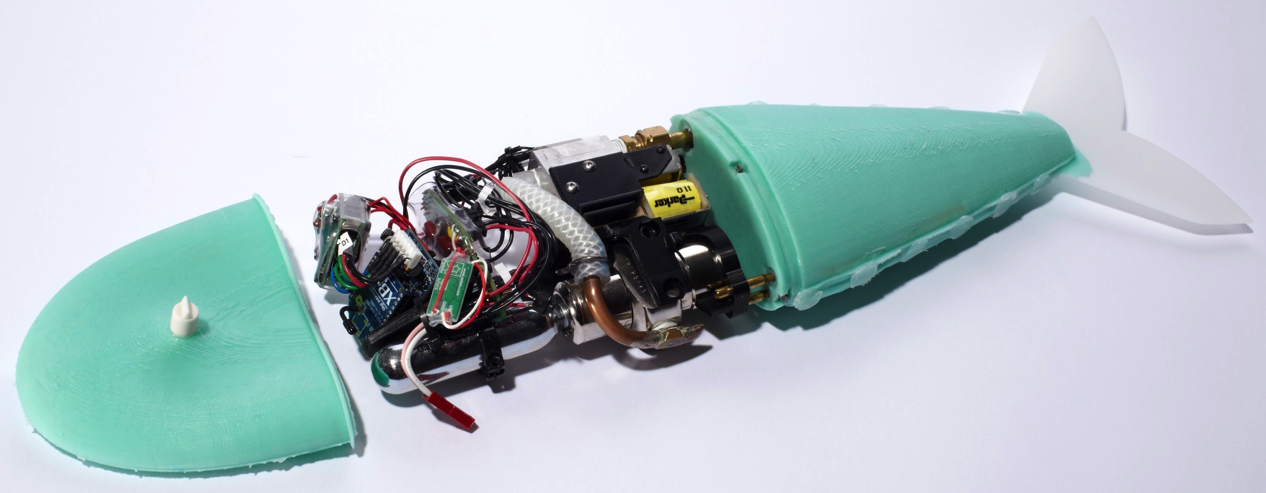
\includegraphics[width=0.9\columnwidth]{Figures/locomotion/pneumaticfish_system.png}
            \caption{}
            \label{fig:pneumaticfish_system}
        \end{subfigure}\\
        \begin{subfigure}[b]{\columnwidth}
            \centering
            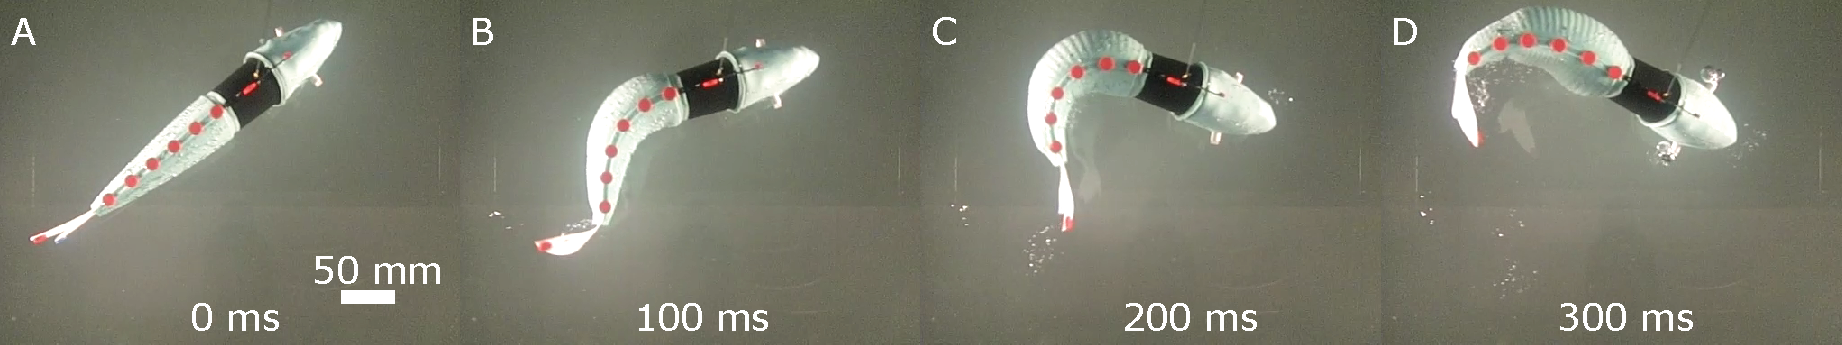
\includegraphics[width=0.9\columnwidth]{Figures/locomotion/pneumaticfish_escape_half.pdf}
            \caption{}
            \label{fig:pneumaticfish_escape}
        \end{subfigure}%
        \caption[Pneumatic Fish.]{A soft pneumatic robotic fish: (\textbf{a}) An overview of the robotic system, photo courtesy of Devon Jarvis, (\textbf{b}) A sequence depicting the fish performing an escape response.}
\end{figure}



\subsection{Hydraulic Fish}
\label{subsec:Locomotion, Hydraulic Fish}
The soft hydraulic fish~\cite{katzschmann2014hydraulic} with a single ribbed actuator is shown as a complete system in Figure~\ref{fig:hydraulic_fish_system_overview}. A close-up view is shown in Figure~\ref{fig:hydraulic_fish_yaw} and the 3d swimming capabilities are shown in Figure~\ref{fig:hydraulic_fish_all_motions}.

\begin{figure}[htb]
        \centering
        \begin{subfigure}[b]{0.48\columnwidth}
            \centering
           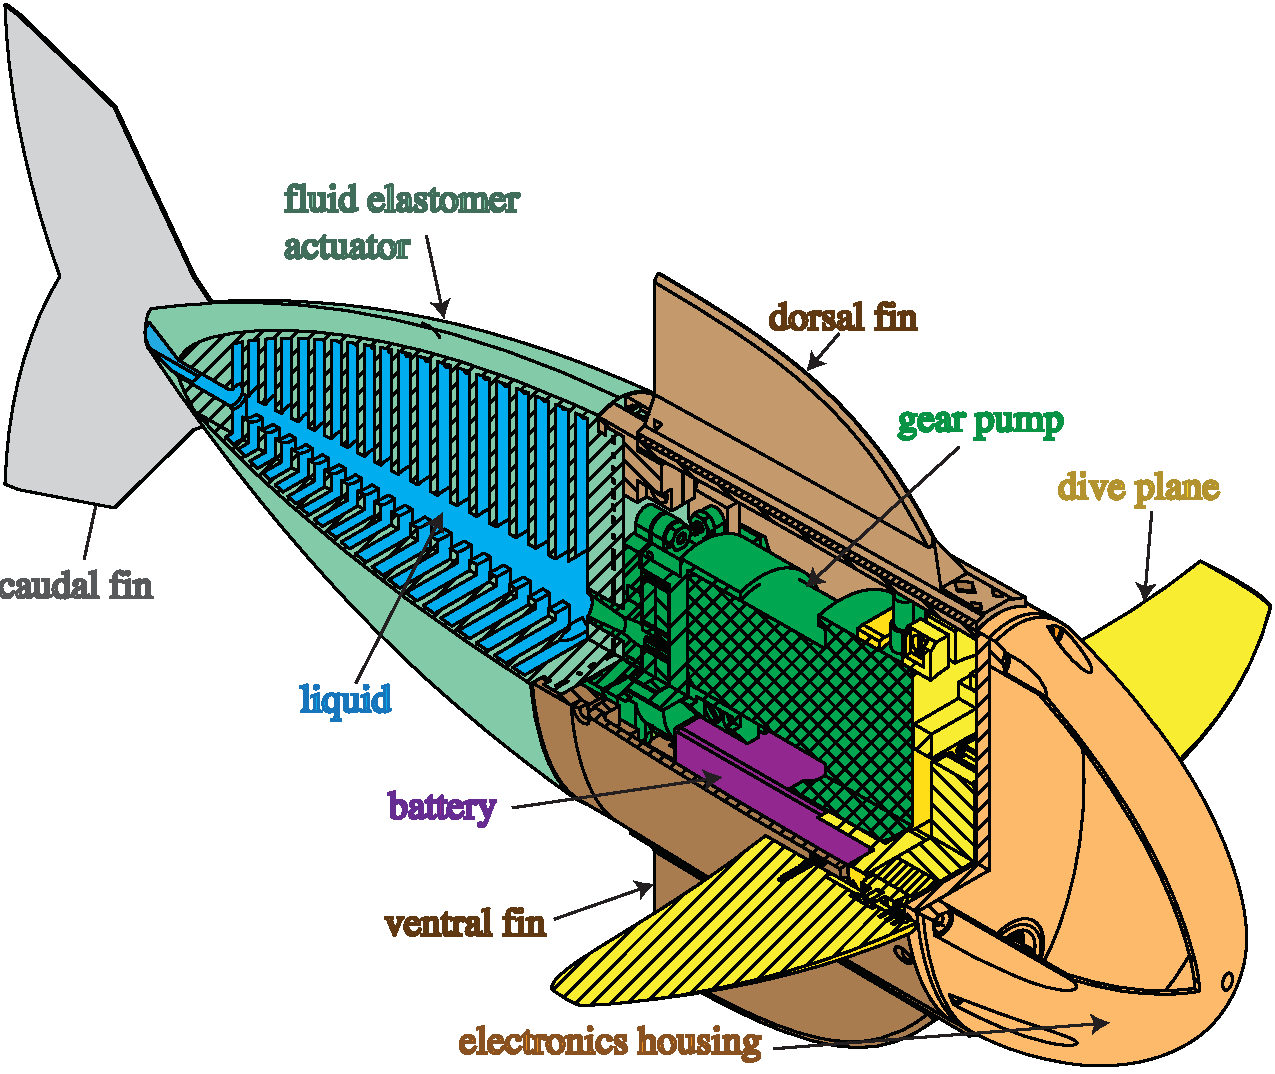
\includegraphics[width=1\columnwidth]{figures/locomotion/hydraulic_fish_system_overview.pdf}
           \caption{}
            \label{fig:hydraulic_fish_system_overview}
        \end{subfigure}
        \begin{subfigure}[b]{0.48\columnwidth}
            \centering
            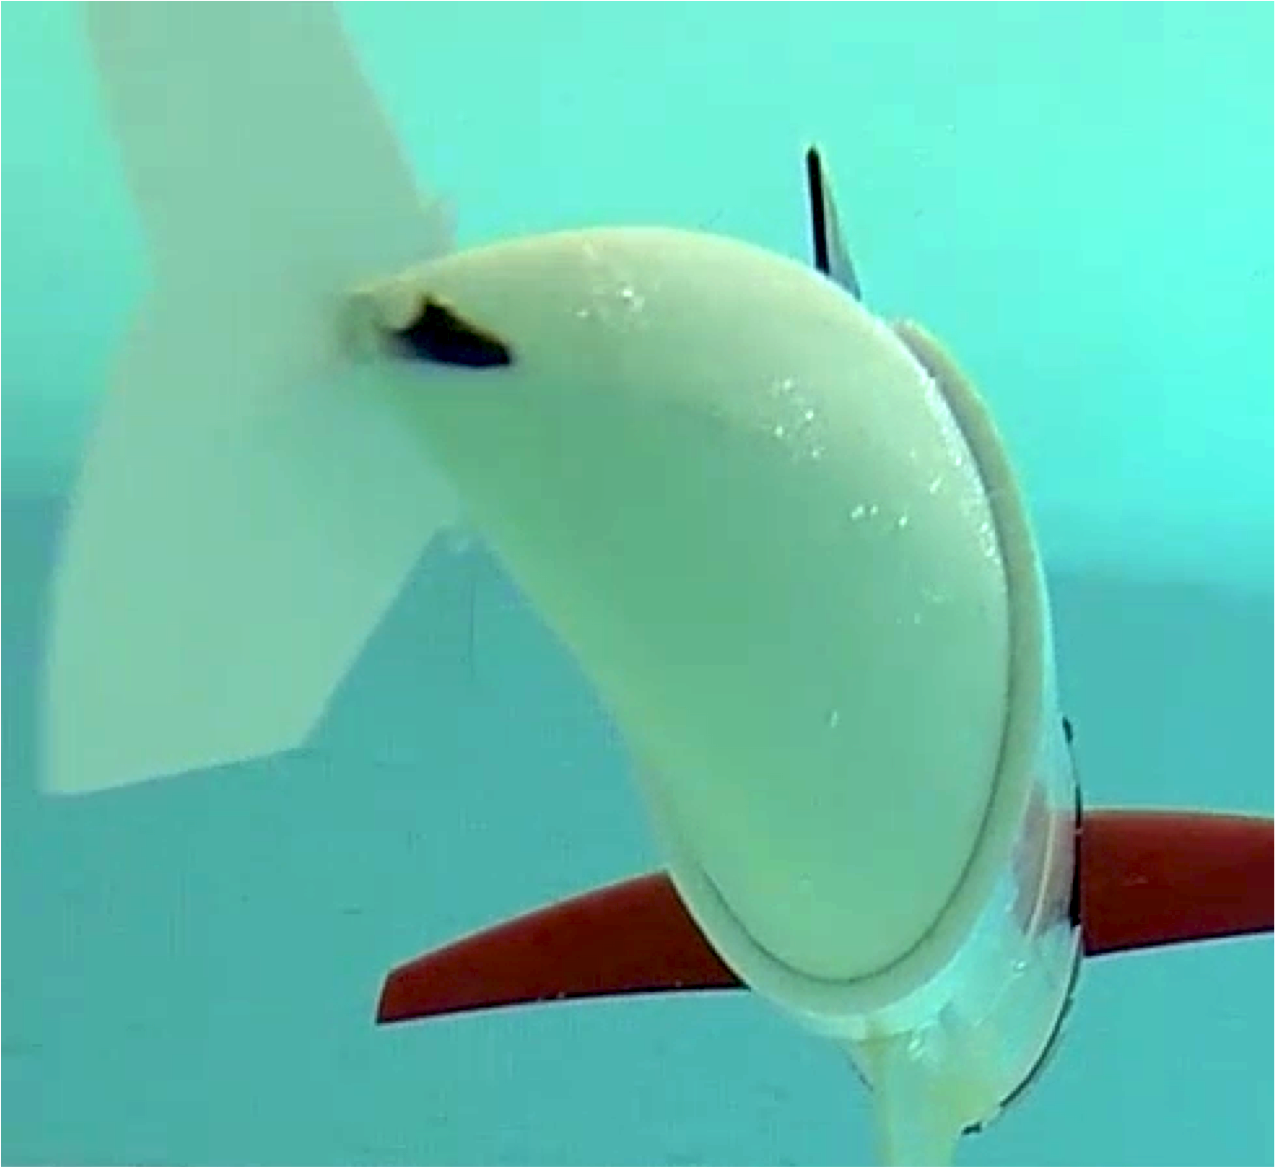
\includegraphics[width=1\columnwidth]{figures/locomotion/hydraulic_fish_yaw.png}
            \caption{}
            \label{fig:hydraulic_fish_yaw}
        \end{subfigure}\\
        \begin{subfigure}[b]{1\columnwidth}
            \centering
            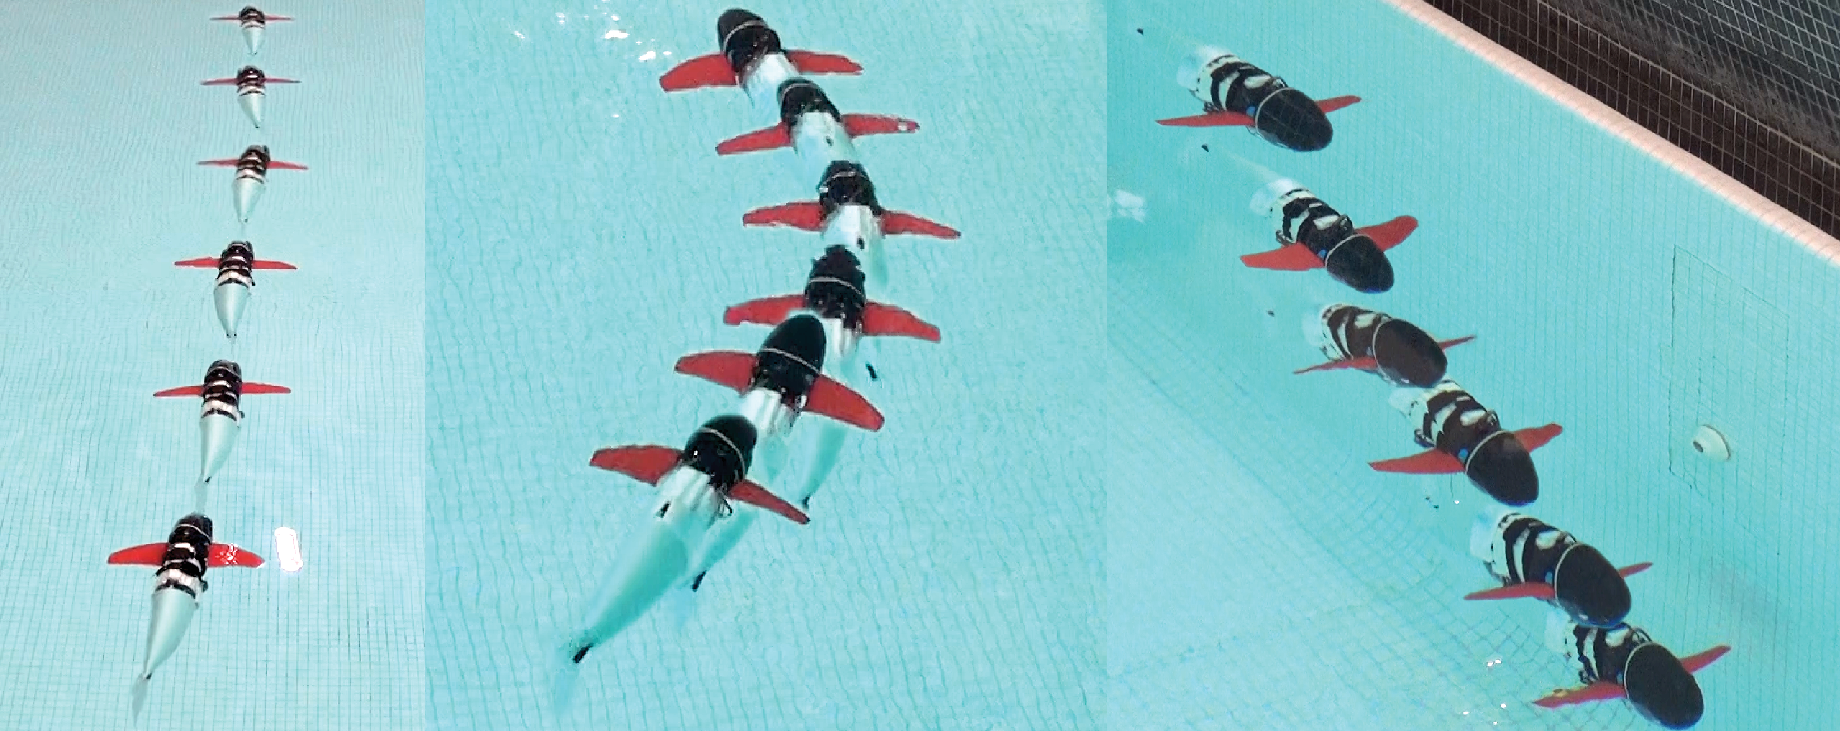
\includegraphics[width=1\columnwidth]{figures/locomotion/hydraulic_fish_all_motions.pdf}
            \caption{}
            \label{fig:hydraulic_fish_all_motions}
        \end{subfigure}%
        \caption[Hydraulic soft robotic fish]{A soft hydraulic robotic fish: (\textbf{a}) A schematic of the system, (\textbf{b}) underwater swimming motion, and (\textbf{c}) example of continuous forward swimming, yaw motion, and diving.}
\end{figure} 